\documentclass[11pt]{article}

\usepackage[margin=1in]{geometry}
\usepackage{amsmath,amssymb,amsfonts,mathtools}
\usepackage{booktabs}
\usepackage{array}
\usepackage{hyperref}
\usepackage{xcolor}
\usepackage{microtype}
\usepackage{tikz}
\usetikzlibrary{arrows.meta,positioning,decorations.pathreplacing,calc,matrix}

\hypersetup{
  colorlinks=true,
  linkcolor=blue!55!black,
  urlcolor=blue!55!black,
  citecolor=blue!55!black
}

\newcommand{\R}{\mathbb R}
\newcommand{\norm}[1]{\left\lVert #1 \right\rVert}
\newcommand{\argmin}{\operatorname*{arg\,min}}
\newcommand{\dd}{\mathrm d}
\newcommand{\Path}{\mathcal P}
\newcommand{\reportbuilddatetime}{2026-05-16 17:02:23 EDT}

\title{Path-Divided-Difference Trend Filtering on Graphs}
\author{\texttt{gflow} graph trend filtering project notes}
\date{Build \reportbuilddatetime}

\begin{document}
\maketitle

\begin{abstract}
This note proposes a path-divided-difference graph trend-filtering penalty for
\texttt{gflow}.  The goal is to keep the essential behavior of classical
one-dimensional trend filtering on path graphs while extending it to metric
graphs with branches.  The central construction is simple: enumerate local
graph paths, turn each path into a one-dimensional coordinate system using edge
lengths, compute the ordinary divided difference along that path, and penalize
the absolute values of those pathwise differences.  The centerpiece is a
three-arm star graph, the smallest example where graph trend filtering must
decide what ``linear'' should mean at a branch point.
\end{abstract}

\section{Purpose}

The current \texttt{gflow} graph trend-filtering implementation follows the
recursive graph-operator construction
\[
  \Delta^{(k+1)}
  =
  \begin{cases}
  L^{(k+1)/2}, & k \text{ odd},\\
  D L^{k/2}, & k \text{ even},
  \end{cases}
\]
where \(D\) is an oriented incidence matrix and \(L=D^TD\) is a graph
Laplacian.  This construction is natural for general graphs, but it does not
reproduce classical one-dimensional trend filtering on a path graph for higher
orders.  In particular, the current graph order-2 operator behaves more like
an edge difference of graph Laplacian values than like the third divided
difference used by one-dimensional quadratic trend filtering.

This document proposes a second operator family:
\[
  \Delta^{(r)}_{G,\mathrm{path}},
\]
where \(r\) is the divided-difference order.  The intended relation to trend
filtering order \(k\) is
\[
  r = k+1.
\]
Thus \(k=0\) penalizes first differences, \(k=1\) penalizes second divided
differences, and \(k=2\) penalizes third divided differences.

\section{Classical Divided Differences}

Let
\[
  t_0 < t_1 < \cdots < t_r
\]
be positions on the real line, and let \(z_j=f(t_j)\).  The first divided
difference is
\[
  [t_0,t_1]f
  =
  \frac{z_1-z_0}{t_1-t_0}.
\]
The second divided difference is
\[
  [t_0,t_1,t_2]f
  =
  \frac{
    [t_1,t_2]f - [t_0,t_1]f
  }{
    t_2-t_0
  }.
\]
Some conventions multiply this expression by \(2\), so that it equals the
ordinary quadratic coefficient scale.  The scaling convention matters for
\(\lambda\), but not for the fitted path after the tuning grid is adjusted.
The third divided difference is defined recursively:
\[
  [t_0,t_1,t_2,t_3]f
  =
  \frac{
    [t_1,t_2,t_3]f - [t_0,t_1,t_2]f
  }{
    t_3-t_0
  }.
\]

The general recursive definition is
\[
  [t_0,\ldots,t_r]f
  =
  \frac{
    [t_1,\ldots,t_r]f - [t_0,\ldots,t_{r-1}]f
  }{
    t_r-t_0
  }.
\]

The key fact is the null-space property:
\[
  [t_0,\ldots,t_r]f=0
  \quad\text{for every consecutive window}
\]
if the sampled values lie on a polynomial of degree at most \(r-1\).
This is the algebra behind one-dimensional trend filtering.

\begin{figure}[ht]
\centering
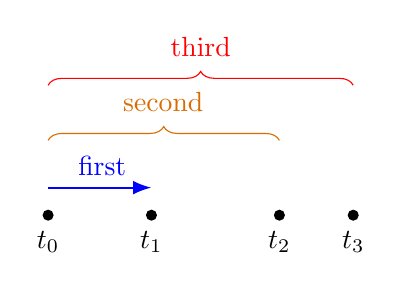
\begin{tikzpicture}[x=1.25cm,y=1cm,>=Latex]
  \foreach \i/\x in {0/0,1/1.05,2/2.35,3/3.1} {
    \fill[black] (\x,0) circle (2pt);
    \node[below] at (\x,-0.08) {\(t_{\i}\)};
  }
  \draw[blue,thick,->] (0,0.35) -- (1.05,0.35);
  \node[blue,above] at (0.55,0.38) {first};
  \draw[orange!85!black,decorate,decoration={brace,amplitude=5pt}]
    (0,0.95) -- (2.35,0.95);
  \node[orange!85!black,above=7pt] at (1.17,0.95) {second};
  \draw[red,decorate,decoration={brace,amplitude=5pt}]
    (0,1.65) -- (3.1,1.65);
  \node[red,above=7pt] at (1.55,1.65) {third};
\end{tikzpicture}
\caption{Divided differences are local polynomial detectors.  A second divided
difference measures curvature; a third divided difference measures change in
curvature.}
\end{figure}

\section{Metric Graphs and Path Coordinates}

Let
\[
  G=(V,E,\ell)
\]
be an undirected graph with positive edge lengths
\[
  \ell_{uv}>0,\qquad (u,v)\in E.
\]
For a simple graph path
\[
  p=(v_0,v_1,\ldots,v_r),
\]
define path-induced coordinates
\[
  t_0=0,\qquad
  t_j=\sum_{m=1}^j \ell_{v_{m-1}v_m},\quad j=1,\ldots,r.
\]
The pathwise divided difference is then
\[
  \Delta^{(r)}_p f
  =
  [t_0,\ldots,t_r]\,
  (f_{v_0},\ldots,f_{v_r}).
\]
This is an ordinary one-dimensional divided difference, but the coordinate
axis is induced by graph edge lengths along the path.

\section{Canonical Path Rows}

For fixed order \(r\), let
\[
  \overrightarrow{\Path}_r(G)
  =
  \{(v_0,\ldots,v_r): v_i \text{ distinct and } (v_{i-1},v_i)\in E\}
\]
be the set of directed simple length-\(r\) paths.  Reversing a path does not
change the absolute value of the divided difference except for an order-
dependent sign.  Since the trend-filtering penalty uses absolute values, the
two rows
\[
  (v_0,\ldots,v_r)
  \quad\text{and}\quad
  (v_r,\ldots,v_0)
\]
are duplicates for penalty purposes.

Define the reversal equivalence relation
\[
  (v_0,\ldots,v_r)\sim(v_r,\ldots,v_0),
\]
and let
\[
  \Path_r^{\mathrm{can}}(G)
  =
  \overrightarrow{\Path}_r(G)/{\sim}
\]
be the canonical undirected path-row set.  In computation, each equivalence
class can be represented by the lexicographically smaller orientation.

This canonicalization has a practical purpose.  On a path graph, classical
one-dimensional trend filtering uses each consecutive window once.  If both
orientations were retained, the penalty would be multiplied by two and the
same numerical \(\lambda\) grid would no longer match the 1D reference solver.

\section{The Path-Divided-Difference Penalty}

The proposed penalty has the form
\[
  \norm{\Delta^{(r)}_{G,\mathrm{path}}f}_1
  =
  \sum_{p\in \Path_r^{\mathrm{can}}(G)}
  w_p
  \left|\Delta^{(r)}_p f\right|.
\]
The weights \(w_p\) are not conductances in the low-pass smoothing sense.
They are row weights for the \(\ell_1\) graph trend-filtering penalty.

\subsection{Unit Weighting}

The simplest choice is
\[
  w_p=1.
\]
This is the natural default when exact path-graph parity is the priority.
On a path graph with vertices ordered along the path, it gives the same rows
as the classical divided-difference trend-filtering operator.

\subsection{Anchor-Mean Weighting}

For graphs with highly unequal branching, one may want to prevent vertices
with many outgoing path continuations from dominating the penalty.  Let
\[
  a(p)
\]
be the first vertex of the chosen canonical representative of \(p\), and let
\[
  \Path_{r,u}^{\mathrm{can}}(G)
  =
  \{p\in \Path_r^{\mathrm{can}}(G): a(p)=u\}.
\]
The anchor-mean choice is
\[
  w_p
  =
  \frac{1}{|\Path_{r,a(p)}^{\mathrm{can}}(G)|}.
\]
The corresponding penalty can be written as
\[
  \norm{\Delta^{(r)}_{G,\mathrm{path}}f}_{1,\mathrm{anchor}}
  =
  \sum_{u\in V}
  \frac{1}{|\Path_{r,u}^{\mathrm{can}}(G)|}
  \sum_{p\in \Path_{r,u}^{\mathrm{can}}(G)}
  \left|\Delta^{(r)}_p f\right|,
\]
with the convention that vertices with no length-\(r\) paths contribute zero.

In an R interface, this suggests
\[
  \texttt{path.weighting = c("unit", "anchor.mean")}.
\]

\section{Exact Agreement on Path Graphs}

Consider a path graph
\[
  1-2-\cdots-n
\]
with edge lengths
\[
  h_i=\ell_{i,i+1}.
\]
The canonical length-\(r\) path rows are exactly
\[
  (1,2,\ldots,r+1),\quad
  (2,3,\ldots,r+2),\quad\ldots,\quad
  (n-r,\ldots,n).
\]
The path-induced coordinates are
\[
  0,\ h_i,\ h_i+h_{i+1},\ \ldots,\ \sum_{m=i}^{i+r-1}h_m.
\]
Therefore
\[
  \Delta^{(r)}_{G,\mathrm{path}}
\]
with unit weighting is exactly the nonuniform one-dimensional
divided-difference operator on the path.

\paragraph{Consequence.}
If \(\texttt{fit.graph.trend.filtering()}\) uses this operator on a path graph,
then order \(k\) graph trend filtering with \(r=k+1\) can be made
algebraically identical to the corresponding \texttt{genlasso} trend filter,
up to the same divided-difference scaling convention and the same
\(\lambda\) selection rule.

\begin{figure}[ht]
\centering
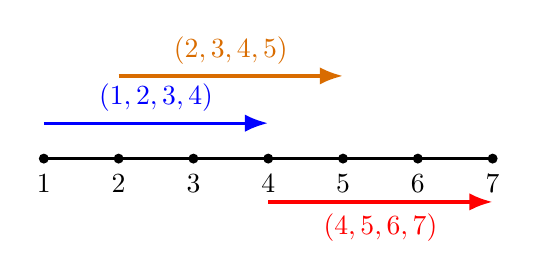
\begin{tikzpicture}[x=0.95cm,y=1cm,>=Latex]
  \foreach \i in {1,...,7} {
    \fill[black] (\i,0) circle (1.8pt);
    \node[below] at (\i,-0.08) {\(\i\)};
  }
  \draw[thick] (1,0) -- (7,0);
  \draw[blue,very thick,->] (1,0.45) -- (4,0.45);
  \node[blue,above] at (2.5,0.47) {\((1,2,3,4)\)};
  \draw[orange!85!black,very thick,->] (2,1.05) -- (5,1.05);
  \node[orange!85!black,above] at (3.5,1.07) {\((2,3,4,5)\)};
  \draw[red,very thick,->] (4,-0.55) -- (7,-0.55);
  \node[red,below] at (5.5,-0.58) {\((4,5,6,7)\)};
\end{tikzpicture}
\caption{For \(r=3\), canonical path rows on a path graph are exactly the
sliding four-point windows of one-dimensional quadratic trend filtering.}
\end{figure}

\section{The Star Graph Is the Key Test Case}

The smallest graph that is not merely a path is a star.  To test an order
\(k=1\) trend filter, whose penalty uses \(r=2\) second divided differences,
the smallest useful star has two vertices on each arm:
\[
  u-v_{a1}-v_{a2},
  \qquad a=1,2,3.
\]
Here \(u\) is the center.  The graph has one shared branch point and three
arms.

\begin{figure}[ht]
\centering
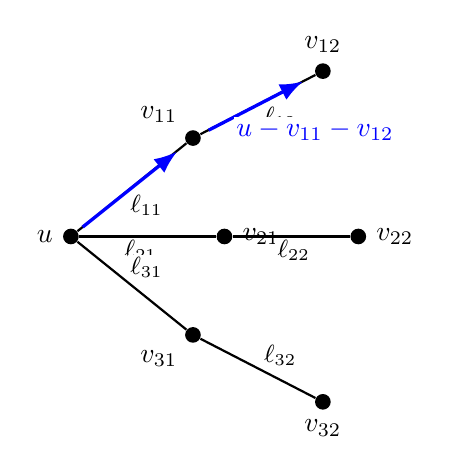
\begin{tikzpicture}[>=Latex,node distance=1cm,
  edge label/.style={font=\small,fill=white,inner sep=1pt}]
  \node[circle,fill=black,inner sep=2pt,label=left:{\(u\)}] (u) at (0,0) {};

  \node[circle,fill=black,inner sep=2pt,label=above left:{\(v_{11}\)}] (v11) at (1.55,1.25) {};
  \node[circle,fill=black,inner sep=2pt,label=above:{\(v_{12}\)}] (v12) at (3.20,2.10) {};
  \draw[thick] (u) -- node[edge label,below right,pos=0.45] {\(\ell_{11}\)} (v11)
    -- node[edge label,below right,pos=0.52] {\(\ell_{12}\)} (v12);

  \node[circle,fill=black,inner sep=2pt,label=right:{\(v_{21}\)}] (v21) at (1.95,0) {};
  \node[circle,fill=black,inner sep=2pt,label=right:{\(v_{22}\)}] (v22) at (3.65,0) {};
  \draw[thick] (u) -- node[edge label,below,pos=0.45] {\(\ell_{21}\)} (v21)
    -- node[edge label,below,pos=0.52] {\(\ell_{22}\)} (v22);

  \node[circle,fill=black,inner sep=2pt,label=below left:{\(v_{31}\)}] (v31) at (1.55,-1.25) {};
  \node[circle,fill=black,inner sep=2pt,label=below:{\(v_{32}\)}] (v32) at (3.20,-2.10) {};
  \draw[thick] (u) -- node[edge label,above right,pos=0.45] {\(\ell_{31}\)} (v31)
    -- node[edge label,above right,pos=0.52] {\(\ell_{32}\)} (v32);

  \draw[blue,very thick,->] (0.15,0.12) -- (1.35,1.08);
  \draw[blue,very thick,->] (1.75,1.35) -- (2.95,1.97);
  \node[blue,fill=white,inner sep=1pt] at (3.10,1.35) {\(u-v_{11}-v_{12}\)};
\end{tikzpicture}
\caption{The three-arm star with two vertices per arm.  It is the simplest
graph where a path-divided-difference penalty must decide whether smoothness
should be enforced along arms, across arms, or both.}
\end{figure}

\subsection{Why Cross-Arm Paths Are Not Innocent}

If we include every simple length-2 path, then paths such as
\[
  v_{11}-u-v_{21}
\]
are included.  With equal edge lengths, zero second difference on all such
cross-arm paths imposes equations like
\[
  f_{11}-2f_u+f_{21}=0.
\]
Combining all cross-arm equations forces compatibility between slopes on
different arms.  On a three-arm star with only one vertex per arm, it can
collapse the order-1 null space to constants.

That may be desirable for some embedded problems, but it is not the desired
first implementation here.  If the graph represents a branching metric object,
then a branch point should share a function value, while each outgoing arm may
have its own slope.

\subsection{Arm-Continuation Paths}

For the first implementation, the intended second-difference paths at the
center are the arm-continuation paths
\[
  (u,v_{11},v_{12}),\qquad
  (u,v_{21},v_{22}),\qquad
  (u,v_{31},v_{32}).
\]
With equal edge lengths, zero second divided difference gives
\[
  f_u - 2f_{11} + f_{12}=0,
\]
\[
  f_u - 2f_{21} + f_{22}=0,
\]
\[
  f_u - 2f_{31} + f_{32}=0.
\]
Equivalently, for each arm \(a\),
\[
  f_{a2}-f_{a1}
  =
  f_{a1}-f_u.
\]
This says that each arm is locally linear as a function of distance from the
center.

\subsection{The Null Space on the Star}

For equal edge lengths, the three equations imply
\[
  f_{a1}=f_u+s_a,
  \qquad
  f_{a2}=f_u+2s_a,
  \qquad a=1,2,3.
\]
Thus the null space has four degrees of freedom:
\[
  f_u,\quad s_1,\quad s_2,\quad s_3.
\]
The center value \(f_u\) is shared, but the three arms may have three
different slopes.

\[
\begin{array}{c|c}
\text{quantity} & \text{meaning}\\
\midrule
f_u & \text{shared intercept at the branch point}\\
s_1 & \text{slope along arm 1}\\
s_2 & \text{slope along arm 2}\\
s_3 & \text{slope along arm 3}
\end{array}
\]

This is the behavior we want the operator to have in the first implementation:
linear along each arm, coupled only through the common value at the branch
point.

\begin{figure}[ht]
\centering
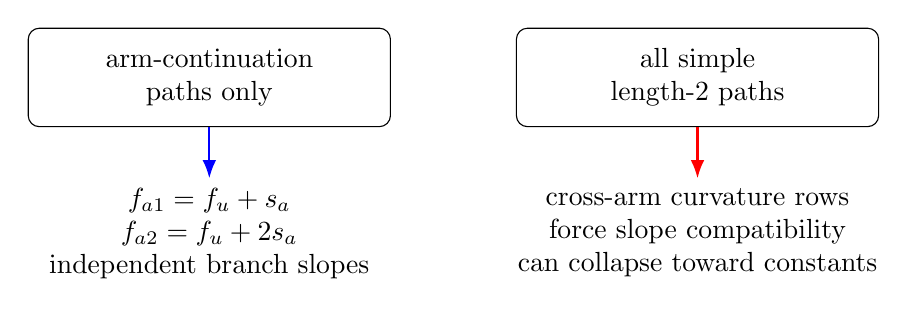
\begin{tikzpicture}[x=1cm,y=1cm,>=Latex]
  \node[draw,rounded corners,align=center,minimum width=4.6cm,minimum height=1.25cm] (arm)
    at (0,0) {arm-continuation\\paths only};
  \node[draw,rounded corners,align=center,minimum width=4.6cm,minimum height=1.25cm] (cross)
    at (6.2,0) {all simple\\length-2 paths};

  \node[align=center,below=0.65cm of arm] (armtext)
    {\(f_{a1}=f_u+s_a\)\\\(f_{a2}=f_u+2s_a\)\\independent branch slopes};
  \node[align=center,below=0.65cm of cross] (crosstext)
    {cross-arm curvature rows\\force slope compatibility\\can collapse toward constants};

  \draw[blue,thick,->] (arm) -- (armtext);
  \draw[red,thick,->] (cross) -- (crosstext);
\end{tikzpicture}
\caption{The star graph exposes the modeling choice.  Arm-continuation paths
preserve branch-specific slopes; all simple paths also penalize turns through
the branch point.}
\end{figure}

\subsection{Unequal Edge Lengths}

Let the two edge lengths on arm \(a\) be
\[
  h_{a1}=\ell_{u,v_{a1}},
  \qquad
  h_{a2}=\ell_{v_{a1},v_{a2}}.
\]
The zero second divided-difference condition along the arm is
\[
  \frac{
    \frac{f_{a2}-f_{a1}}{h_{a2}}
    -
    \frac{f_{a1}-f_u}{h_{a1}}
  }{
    h_{a1}+h_{a2}
  }
  =0.
\]
Therefore
\[
  \frac{f_{a2}-f_{a1}}{h_{a2}}
  =
  \frac{f_{a1}-f_u}{h_{a1}}.
\]
The slope along arm \(a\) is constant in metric distance, but the slopes may
still differ across arms.

\section{A First Implementation Path Family}

The star example shows that path enumeration is not merely an implementation
detail.  The first implementation should therefore use a deliberate path
family rather than blindly using every simple path.

For the initial \texttt{gflow} implementation, define
\[
  \Path_r^{\mathrm{branch}}(G)
  \subseteq
  \Path_r^{\mathrm{can}}(G)
\]
to contain canonical paths that continue along a local branch rather than
turning through a high-degree vertex.  On a path graph,
\[
  \Path_r^{\mathrm{branch}}(G)
  =
  \Path_r^{\mathrm{can}}(G),
\]
so exact 1D parity is preserved.  On a star, length-2 rows include arm
continuations such as
\[
  u-v_{a1}-v_{a2},
\]
but exclude cross-arm rows such as
\[
  v_{a1}-u-v_{b1},\qquad a\ne b.
\]

This suggests an implementation option:
\[
\begin{split}
  &\texttt{operator.family = "path.divided.difference"},\\
  &\texttt{path.family = c("branch.continuation", "all.simple")},\\
  &\texttt{path.weighting = c("unit", "anchor.mean")}.
\end{split}
\]
The recommended first default is
\[
  \texttt{path.family = "branch.continuation"},
  \qquad
  \texttt{path.weighting = "unit"}.
\]

\section{Estimator}

Given a selected path family \(\Path_r^\star(G)\), the estimator is
\[
  \widehat f_\lambda
  =
  \argmin_{f\in\R^{|V|}}
  \left\{
    \frac12\norm{y-f}_2^2
    +
    \lambda
    \sum_{p\in \Path_r^\star(G)}
    w_p|\Delta^{(r)}_p f|
  \right\}.
\]
Equivalently, if \(A_{r,\mathrm{path}}\) is the sparse matrix whose rows are
the weighted divided-difference path rows, then
\[
  \widehat f_\lambda
  =
  \argmin_f
  \left\{
    \frac12\norm{y-f}_2^2
    +
    \lambda\norm{A_{r,\mathrm{path}}f}_1
  \right\}.
\]

This is a generalized lasso problem.  It can use the same broad computational
framework as the current \texttt{fit.graph.trend.filtering()} implementation,
provided the penalty matrix can be constructed and passed to the solver.

\section{Comparison With Recursive Graph Trend Filtering}

The recursive graph operator and the path-divided-difference operator encode
different meanings of smoothness.

\[
\begin{array}{p{0.38\linewidth}p{0.48\linewidth}}
\toprule
\textbf{Recursive graph operator} & \textbf{Path-divided-difference operator}\\
\midrule
Uses incidence and Laplacian powers. &
Uses ordinary divided differences along selected graph paths.\\
Natural from graph calculus. &
Natural from metric path geometry.\\
On a path, higher orders need not match classical 1D trend filtering. &
On a path, unit-weighted canonical rows reproduce classical 1D trend filtering.\\
Branch behavior is determined by \(D\) and \(L\). &
Branch behavior is determined by the chosen path family.\\
\bottomrule
\end{array}
\]

The important point is not that one construction is universally better.  They
are different modeling assumptions.  The path-divided-difference construction
is designed for experiments where graph edges are interpreted as metric
segments and smoothness should be measured along local graph paths.

\section{Testing Implications}

The proposed operator family has unusually clear tests.

\paragraph{Path parity tests.}
On path graphs with unit weighting, compare the constructed penalty matrix
against the one-dimensional divided-difference matrix used by a reference
implementation.  This should be tested for equal and unequal edge lengths.

\paragraph{Canonicalization tests.}
Verify that a path and its reverse produce only one row.  This prevents
accidental doubling of the penalty and keeps the \(\lambda\) scale comparable
to one-dimensional trend filtering.

\paragraph{Star null-space tests.}
For the three-arm star with two vertices per arm, the \(r=2\)
branch-continuation operator should annihilate vectors satisfying
\[
  f_{a1}=f_u+s_a,\qquad f_{a2}=f_u+2s_a.
\]
It should not force \(s_1=s_2=s_3\).

\paragraph{Cross-arm contrast tests.}
If \(\texttt{path.family = "all.simple"}\) is implemented, it should include
cross-arm rows and therefore have a different null space on the star graph.
This contrast is a useful guard against silently changing the branch-continuity
semantics.

\section{Open Modeling Questions}

Several choices should remain explicit until empirical benchmarks and small
graph algebra agree.

\begin{enumerate}
  \item Should \(\texttt{path.weighting = "unit"}\) remain the default because
        it gives the cleanest 1D parity?
  \item Should \(\texttt{path.family = "branch.continuation"}\) be the default
        for metric graph data?
  \item How should branch-continuation paths be detected in graphs with cycles,
        noisy neighborhoods, or no obvious arm structure?
  \item Should cross-arm paths be available as an explicit stronger-smoothness
        option?
  \item For higher orders, should the first implementation limit \(r\) to
        \(1,2,3\), where path enumeration and diagnostics remain transparent?
\end{enumerate}

\section{Summary}

The path-divided-difference graph trend-filtering penalty is built from local
one-dimensional divided differences along selected graph paths:
\[
  \norm{\Delta^{(r)}_{G,\mathrm{path}}f}_1
  =
  \sum_{p\in\Path_r^\star(G)}
  w_p|\Delta^{(r)}_p f|.
\]
With canonical path rows and unit weighting, it reproduces ordinary
one-dimensional trend filtering on path graphs.  On branched graphs, the
selected path family becomes the modeling decision.  The three-arm star shows
why this matters: branch-continuation paths allow one shared center value and
independent arm slopes, while all simple paths impose stronger cross-arm
compatibility.  This makes the star graph the natural first analytic and unit
test for the proposed \texttt{gflow} operator family.

\end{document}
